%!TEX root = ../report.tex
\chapter{Analysis}\label{ch:analysis}

This chapter is going to show all analysis artefacts regarding Trale Messenger project.

\section{Actors}\label{sec:actors}

Our system is in interaction with two actors - the user and the admin.
The user is the key person interacting with the system and the chat client itself.
The admin is the person interacting with the admin panel to configure several settings and monitoring the chat server.
Figure~\ref{tab:table23} is a mapping of all use cases and the corresponding actor.

\begin{table}[ht]
    \centering
    \begin{tabular}[t]{@{}|l|l|l|@{}}
        \toprule
        \textbf{Actor} &
        \textbf{Description} &
        \textbf{List of related use cases} \\
        \midrule
        User &
        \parbox[t]{2.2cm}{An end-user of the Trale Messenger app} &
        \begin{tabular}[t]{@{}l@{}}
            register,  login,  send message,  logout,  search user,  block user,\\
            change settings,  toggle read receipt,  set profile picture,\\
            view profile picture,  open chat,  start new chat,  send voice message,\\
            send file,  delete message,  delete conversation,  star message
        \end{tabular} \\
        \hline
        Admin &
        \parbox[t]{2.2cm}{An administrator of a Trale server system} &
        \begin{tabular}[t]{@{}l@{}}
            \textbf{Settings Service:} \\
            change settings, add report reason, ban user, block user, login,\\
            create report reason, edit report reason, generate invite,\\
            get all report reasons, remove invite code,\\
            \\ \textbf{Reporting Service:}\\
            delete report reason, remove report reason,\\
            select all report reasons, update report reason, require invite,\\
            require e-mail confirmation, require 2FA,\\
            \\ \textbf{Identity Service:}\\
            add invite code, delete invite code, select all invite code
        \end{tabular} \\
        \bottomrule
    \end{tabular}
    \caption{List of use cases per actor}
    \label{tab:table23}
\end{table}

\section{Use Case Diagram}\label{sec:use-case-diagram}

\begin{figure}[H]
  \vspace{-2em}
  \caption{Use case diagram Trale Messenger}
  \centering
  \def
  % \svgwidth{15cm}
  \svgscale{.7}
  \input{./graphics/usecase-diagram.pdf_tex}
  \label{fig:figure}
\end{figure}

\section{Entity relationship diagram (ERD)}\label{sec:entity-relationship-diagram-(erd)}

\begin{figure}[H]
    \caption{Entity relationship diagram (ERD)}
    \centering
    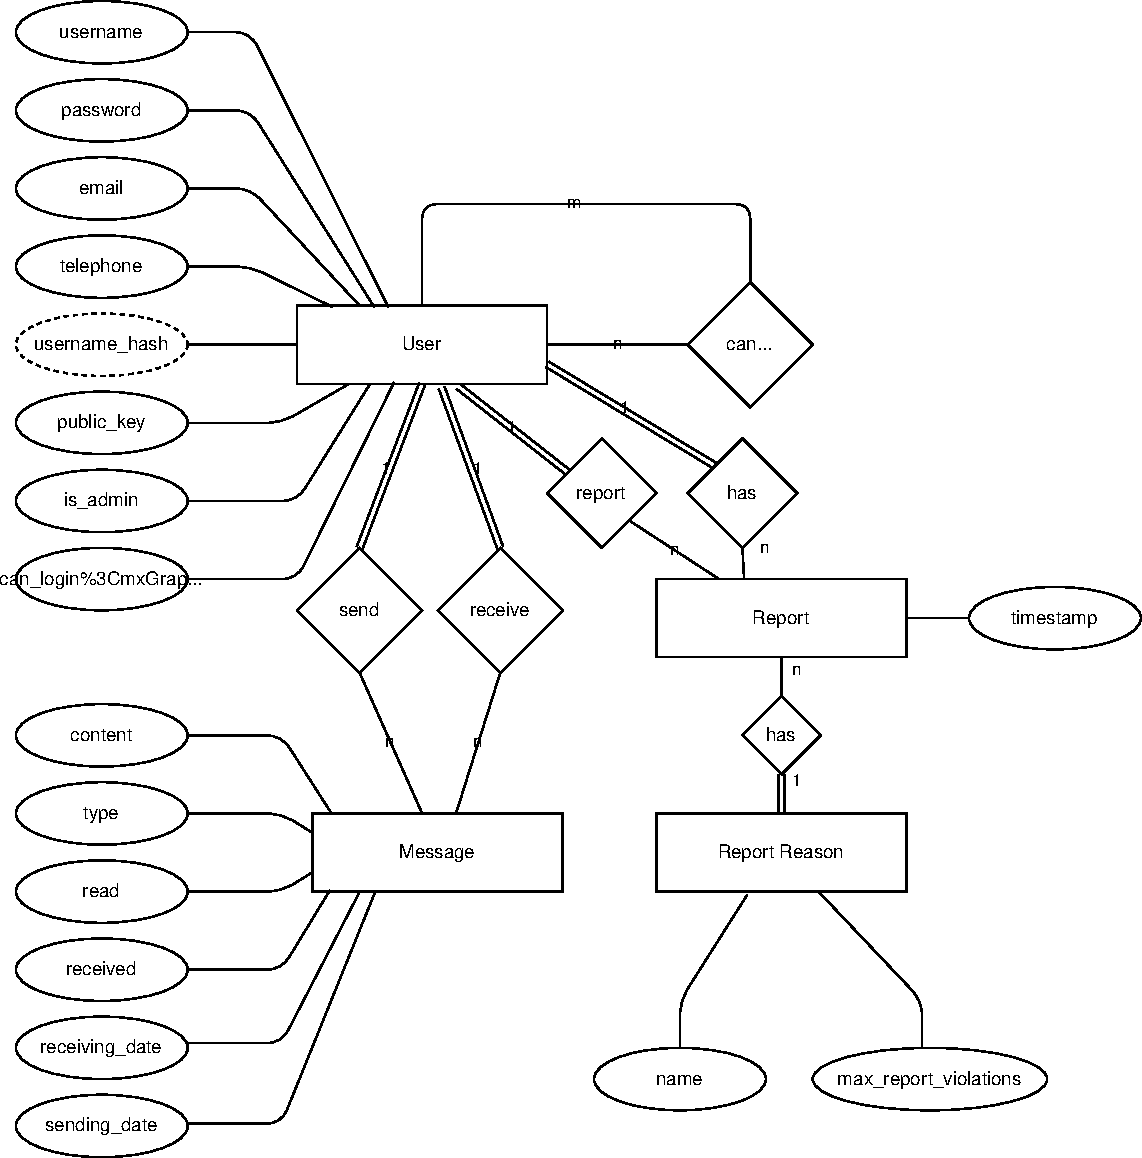
\includegraphics[width=17cm]{./graphics/er-model}
    \label{fig:figure31}
\end{figure}
